%==========================================================================
% D-RECIPE: Dynamic Continual Learning for Temporal Knowledge Graph
%           Forecasting with Incremental Rule Mining and LLM Adaptation
%
% Authors: Busisani Mac Dube, Jean Vincent Fonou Dombeu
% Draft — 2026
%==========================================================================
\documentclass[10pt,twocolumn]{article}

%----------------------------------------------------------------------
% Packages
%----------------------------------------------------------------------
\usepackage[utf8]{inputenc}
\usepackage[T1]{fontenc}
\usepackage{lmodern}
\usepackage[margin=1in]{geometry}
\usepackage{amsmath,amssymb,amsthm}
\usepackage{mathtools}
\usepackage{bm}
\usepackage{graphicx}
\usepackage{booktabs}
\usepackage{multirow}
\usepackage{array}
\usepackage{xcolor}
\usepackage{hyperref}
\usepackage{cleveref}
\usepackage{enumitem}
\usepackage{tikz}
\usepackage{pgfplots}
\pgfplotsset{compat=1.18}
\usetikzlibrary{shapes.geometric, arrows.meta, positioning, fit, backgrounds,
                decorations.pathreplacing, calc}
\usepackage{subcaption}
\usepackage{algorithm}
\usepackage{algpseudocode}
\usepackage{natbib}
\usepackage{microtype}
\usepackage{url}
\usepackage{caption}

%----------------------------------------------------------------------
% Colours
%----------------------------------------------------------------------
\definecolor{drecipeblue}{RGB}{31,119,180}
\definecolor{recipeorange}{RGB}{255,127,14}
\definecolor{naivered}{RGB}{214,39,40}
\definecolor{nodeblue}{RGB}{173,216,230}
\definecolor{nodegray}{RGB}{211,211,211}
\definecolor{nodesoftblue}{RGB}{208,228,244}
\definecolor{nodeyellow}{RGB}{255,239,179}
\definecolor{headerblue}{RGB}{44,62,80}
\definecolor{highlightblue}{RGB}{214,234,248}

%----------------------------------------------------------------------
% Theorem environments
%----------------------------------------------------------------------
\theoremstyle{definition}
\newtheorem{definition}{Definition}
\newtheorem{theorem}{Theorem}
\newtheorem{proposition}{Proposition}

%----------------------------------------------------------------------
% Custom commands
%----------------------------------------------------------------------
\newcommand{\drecipe}{\textsc{D-Recipe}}
\newcommand{\recipe}{\textsc{Recipe-TKG}}
\newcommand{\bfx}{\mathbf{x}}
\newcommand{\bfh}{\mathbf{h}}
\newcommand{\bftheta}{\bm{\theta}}
\newcommand{\calG}{\mathcal{G}}
\newcommand{\calE}{\mathcal{E}}
\newcommand{\calR}{\mathcal{R}}
\newcommand{\calT}{\mathcal{T}}
\newcommand{\calF}{\mathcal{F}}
\newcommand{\calB}{\mathcal{B}}
\newcommand{\calL}{\mathcal{L}}

%----------------------------------------------------------------------
% Metadata
%----------------------------------------------------------------------
\hypersetup{
  pdftitle={D-RECIPE: Dynamic Continual Learning for Temporal Knowledge Graph Forecasting},
  pdfauthor={Busisani Mac Dube, Jean Vincent Fonou Dombeu},
  colorlinks=true,
  linkcolor=drecipeblue,
  citecolor=drecipeblue,
  urlcolor=drecipeblue,
}

%==========================================================================
\begin{document}

%----------------------------------------------------------------------
% Title block
%----------------------------------------------------------------------
\title{%
  \large\bfseries
  D-RECIPE: Dynamic Continual Learning for\\
  Temporal Knowledge Graph Forecasting via\\
  Incremental Rule Mining and LLM Adaptation%
}

\author{
  Busisani Mac Dube\textsuperscript{1} \quad Jean Vincent Fonou Dombeu\textsuperscript{1}\\[4pt]
  \textsuperscript{1}Department of Computer Science, North-West University, South Africa\\[2pt]
  \small\texttt{\{busisani.macdube, jvfonou\}@nwu.ac.za}
}

\date{\small Draft — \today{} \quad [\,arXiv pre-print\,]}

\maketitle
\thispagestyle{empty}

%==========================================================================
\begin{abstract}
%==========================================================================
\noindent
\emph{``The dynamic nature of knowledge poses a challenge, as KGs must
continuously evolve to reflect changes in the world. Most existing work
assumes static KGs, neglecting the continuous addition of new edges and the
modification of existing relationships''}~\citep{MacDube2023review}.
Temporal Knowledge Graph (TKG) forecasting---predicting future facts given a
history of time-stamped events---has seen remarkable progress with rule-based
and large language model (LLM)-based approaches.
However, virtually all existing methods, including the recent state-of-the-art
\recipe{}~\citep{Akgul2025recipe}, treat the KG as a static snapshot:
they require full re-training and full rule re-mining when the graph changes,
making them fundamentally incompatible with real-world deployment scenarios
where edges arrive continuously as a stream.

We introduce \drecipe{} (\textbf{D}ynamic \textbf{R}ule-bas\textbf{E}d
\textbf{C}ont\textbf{I}nual \textbf{P}r\textbf{E}dictor), the first
LLM-based continual TKG completion framework that handles streaming edge
ingestion without offline reprocessing.
\drecipe{} extends \recipe{} with five novel components:
(1)~an \emph{incremental rule miner} that updates temporal rules in $O(k)$
per new edge without full re-mining;
(2)~an \emph{edge stream processor} with $O(1)$ adjacency updates and
emergence detection;
(3)~a \emph{continual learning framework} combining Elastic Weight
Consolidation (EWC), knowledge distillation (KD), and experience replay to
prevent catastrophic forgetting;
(4)~an \emph{adaptive Rule-Based Multi-Hop (RBMH) sampler} with incremental
hop-cache invalidation; and
(5)~full Apple M-series (MPS) hardware compatibility.
Evaluated across four standard TKG benchmarks (ICEWS14, ICEWS18, GDELT,
YAGO), \drecipe{} achieves Hits@10 of 0.681, 0.543, 0.349, and 0.945,
surpassing \recipe{} by up to $+8.4\%$ in the streaming setting.
Continual learning metrics confirm near-zero backward transfer
(BWT~$=+0.005$, ICEWS14), demonstrating that temporal knowledge is preserved
as the graph evolves.
\end{abstract}

\smallskip
\noindent\textbf{Keywords:}
Temporal Knowledge Graphs, Continual Learning, LLM Fine-tuning, Rule Mining,
Knowledge Graph Completion, Catastrophic Forgetting, Streaming Graphs.

%==========================================================================
\section{Introduction}
\label{sec:intro}
%==========================================================================

Knowledge Graphs (KGs) encode world knowledge as triples $(s, r, o)$---
subject, relation, object---enabling downstream reasoning, question answering,
and recommendation~\citep{Hogan2021kg}.
\emph{Temporal} KGs (TKGs) extend this representation to quadruples
$(s, r, o, t)$ capturing events timestamped with a discrete time step $t$.
TKG \emph{forecasting}---predicting future facts from historical
context---is a practically important task underpinning event prediction in
geopolitical analysis (ICEWS, GDELT), encyclopaedic knowledge maintenance
(YAGO), and scientific knowledge evolution.

Despite rapid progress~\citep{Li2021regcn,Sun2021timetraveler,
Liao2024gentkg,Akgul2025recipe}, the field operates under a critical
assumption: \emph{the graph is static}.
Rule mining is performed once on the full training set; LLMs are fine-tuned
on a fixed corpus; evaluation is done on a snapshot.
Yet real TKGs are inherently dynamic---new entities emerge daily, relations
are asserted and retracted, and temporal patterns shift.
As noted by~\citet{MacDube2023review}, this static assumption is a
fundamental gap in the literature.
The naive solution---rerun everything when the graph changes---is
computationally prohibitive.
Full TLogic rule mining~\citep{Liu2022tlogic} on ICEWS14 takes $\approx$8
minutes per update; full fine-tuning of a 7B-parameter LLM takes hours.

\medskip
\noindent\textbf{This paper} closes the gap with \drecipe{}: a framework that
makes LLM-based TKG forecasting compatible with streaming graphs via
principled continual learning.
\drecipe{} is built on \recipe{}~\citep{Akgul2025recipe} and retains all of
its inductive components while adding the machinery needed for
streaming operation.

\medskip
\noindent\textbf{Main Contributions.}\quad
\begin{enumerate}[leftmargin=1.5em,itemsep=2pt,topsep=4pt]
  \item \textbf{Incremental Rule Mining.} We derive an $O(k)$ update rule for
        temporal rule confidence that eliminates full re-mining when new edges
        arrive (\cref{sec:incr_rules}).
  \item \textbf{Edge Stream Processor.} An $O(1)$ adjacency-list-based stream
        processor that tracks entity/relation emergence and supports
        time-bucketed snapshot queries (\cref{sec:stream}).
  \item \textbf{Continual Learning Framework.} A multi-objective loss
        $\calL = \calL_{\text{CE}} + \alpha\calL_C + \beta\calL_{\text{EWC}}
        + \gamma\calL_{\text{KD}}$
        combining cross-entropy, contrastive, EWC, and knowledge distillation
        terms with reservoir-sampled experience replay to prevent catastrophic
        forgetting (\cref{sec:cl}).
  \item \textbf{Adaptive RBMH Sampler.} Dynamic hop-distance recalculation
        with incremental cache invalidation for the subgraph affected by each
        new edge, retaining $\recipe{}$'s rule-guided composite weights
        (\cref{sec:sampler}).
  \item \textbf{Full Apple Silicon (MPS) Compatibility.} Device-agnostic
        BF16 precision training, replacing CUDA-only bitsandbytes quantisation,
        enabling experiments on M-series Macs without modification
        (\cref{sec:impl}).
\end{enumerate}

%==========================================================================
\section{Related Work}
\label{sec:related}
%==========================================================================

\subsection{Temporal Knowledge Graph Completion}

Early TKG methods such as RE-GCN~\citep{Li2021regcn} and
xERTE~\citep{Han2020xerte} model entity evolution with graph neural networks
and temporal attention, respectively.
TANGO~\citep{Han2021tango} uses neural ordinary differential equations to
continuously model temporal graph dynamics; however, all of these methods
treat the training-time graph as fixed.
TimeTraveler~\citep{Sun2021timetraveler} introduces reinforcement learning for
search-path reasoning over snapshots.
TLogic~\citep{Liu2022tlogic} mines temporal Horn rules and uses them for
explicit multi-step reasoning, but rule mining scales quadratically with
graph size and must be re-run on any change.

\subsection{LLM-Based TKG Forecasting}

In-Context Learning (ICL) approaches~\citep{Xiong2024icl} prompt frozen LLMs
with historical facts as context; GenTKG~\citep{Liao2024gentkg} combines
rule retrieval with in-context few-shot prompting.
\recipe{}~\citep{Akgul2025recipe} achieves state-of-the-art results by
combining (i)~Rule-Based Multi-Hop retrieval (RBMH) for context sampling,
(ii)~contrastive LoRA fine-tuning, and (iii)~semantic test-time filtering.
Its explicit limitation---``Rule mining must be rerun if the graph
changes''---directly motivates this work.

\subsection{Continual Learning}

Catastrophic forgetting~\citep{McCloskey1989catastrophic} is the central
challenge in continual learning (CL).
Elastic Weight Consolidation (EWC)~\citep{Kirkpatrick2017ewc} penalises
changes to parameters that are important for previous tasks, quantified via
the Fisher information matrix.
Knowledge Distillation~\citep{Hinton2015distillation} preserves soft
predictions of a frozen teacher as new tasks are learned.
Experience Replay~\citep{Robins1995replay} mitigates forgetting by
interleaving past examples with new ones.
Our framework combines all three mechanisms, adapting them to the
structured-prediction setting of TKG forecasting.
Recent work on continual KG embedding~\citep{Liu2021ckge} focuses on static
triple completion; we are, to our knowledge, the first to apply CL to
LLM-based \emph{temporal} link prediction.

\subsection{Streaming / Incremental KG Methods}

StreamE~\citep{Luo2023streame} proposes streaming embeddings for KGs but does
not handle temporal reasoning rules or LLM integration.
Incremental rule learning for static KGs has been studied in the ILP
community~\citep{Galárraga2013amie}; we adapt this idea to \emph{temporal}
confidence updates under a streaming model.

%==========================================================================
\section{Preliminaries and Problem Formulation}
\label{sec:prelim}
%==========================================================================

\begin{definition}[Temporal Knowledge Graph]
A \emph{Temporal Knowledge Graph} is a set
$\calG = \{(s, r, o, t) \mid s, o \in \calE,\; r \in \calR,\; t \in \calT\}$
where $\calE$ is the entity set, $\calR$ the relation set, and
$\calT \subset \mathbb{Z}^+$ discrete timestamps.
\end{definition}

\begin{definition}[Temporal Link Prediction]
Given a query $(s_q, r_q, ?, t_q)$ with $t_q > \max\calT$, rank all entities
$e \in \calE$ by $P(o = e \mid s_q, r_q, t_q, \calG)$.
Performance is measured by Hits@$k$ (fraction of queries where the true
object is in the top-$k$ predictions) and MRR.
\end{definition}

\begin{definition}[Streaming TKG]
A \emph{streaming TKG} partitions facts into ordered chunks
$\calG = \calG_1 \cup \calG_2 \cup \cdots \cup \calG_N$, where
$\max_{(s,r,o,t)\in\calG_i} t < \min_{(s,r,o,t)\in\calG_{i+1}} t$.
At period $i$, only $\calG_1 \cup \cdots \cup \calG_i$ is observed;
predictions are made for queries at $t > \max_i$.
\end{definition}

\begin{definition}[Continual TKG Forecasting]
A \emph{continual TKG forecasting} system must maintain a predictor $f_\theta$
that, at each period $i$, (a)~ingests $\calG_i$ online, (b)~updates $\theta$
without full reprocessing of $\calG_{<i}$, and (c)~improves (or does not
degrade) Hits@$k$ on queries at $t > i$.
\end{definition}

\medskip
\noindent\textbf{Continual Learning Metrics.}\quad
Following~\citet{Lopez2017gem}, we measure:
\begin{align}
\text{BWT} &= \frac{1}{T-1}\sum_{i=1}^{T-1}
              \bigl(A_{T,i} - A_{i,i}\bigr), \label{eq:bwt}\\
\text{FWT} &= \frac{1}{T-1}\sum_{i=2}^{T}
              \bigl(A_{i-1,i} - \hat{b}_i\bigr), \label{eq:fwt}\\
\text{AvgAcc} &= \frac{1}{T}\sum_{i=1}^{T} A_{T,i}, \label{eq:avgacc}
\end{align}
where $A_{j,i}$ is Hits@10 evaluated on period $i$ after training on period
$j$, and $\hat{b}_i$ is a random-initialisation baseline for period $i$.
BWT~$\approx 0$ (no forgetting); BWT~$< 0$ (catastrophic forgetting);
FWT~$> 0$ (positive forward transfer).

%==========================================================================
\section{D-RECIPE Architecture}
\label{sec:method}
%==========================================================================

\Cref{fig:arch} illustrates the full \drecipe{} pipeline.
At each streaming step, incoming edges $\{(s,r,o,t)\}$ flow through five
sequential components before being used to update the LLM-based predictor.

%----------------------------------------------------------------------
\begin{figure*}[t]
\centering
\begin{tikzpicture}[
    node distance=0.55cm and 0.3cm,
    box/.style={draw, rounded corners=4pt, minimum width=3.6cm,
                minimum height=0.9cm, align=center, font=\small,
                text width=3.4cm},
    arrow/.style={-Stealth, thick, color=drecipeblue},
    label/.style={font=\scriptsize\itshape, text=gray},
    startstop/.style={box, fill=nodeblue!60, draw=drecipeblue, thick},
    process/.style={box, fill=nodesoftblue!60, draw=drecipeblue},
    clbox/.style={box, fill=nodeyellow!70, draw=recipeorange, thick,
                  minimum width=5.0cm, text width=4.8cm},
    output/.style={box, fill=green!15, draw=green!60!black, thick},
]

% ── Column A: input stream ─────────────────────────────────────────────
\node[startstop]               (stream)
      {\textbf{Edge Stream}\\\small$(s,r,o,t)$ batches};

% ── Column B: stream processor ────────────────────────────────────────
\node[process, right=1.4cm of stream] (proc)
      {\textbf{Stream Processor}\\
       \tiny $O(1)$ adjacency update\\
       Entity/relation emergence};

% ── Column C: rule miner ──────────────────────────────────────────────
\node[process, right=1.0cm of proc]   (rules)
      {\textbf{Incremental}\\
       \textbf{Rule Miner}\\
       \tiny $O(k)$ confidence update};

% ── Column D: sampler ─────────────────────────────────────────────────
\node[process, right=1.0cm of rules]  (sampler)
      {\textbf{Adaptive RBMH}\\
       \textbf{Sampler}\\
       \tiny $w = w_n\cdot w_f\cdot(w_t{+}w_c{+}w_{cp})$};

% ── Row 2: LLM + CL ───────────────────────────────────────────────────
\node[process, below=1.2cm of sampler] (llm)
      {\textbf{LLaMA-2-7B / 3-8B}\\
       \textbf{+ LoRA}\\
       \tiny BF16 · MPS/CUDA/CPU};

\node[clbox, below=1.2cm of rules]   (cl)
      {\textbf{Continual Learner}\\[2pt]
       \tiny
       $\calL = \calL_{\text{CE}}
                + \alpha\calL_C
                + \beta\calL_{\text{EWC}}
                + \gamma\calL_{\text{KD}}$\\[2pt]
       EWC (Fisher regularisation)\\
       KD (frozen teacher snapshot)\\
       Replay (reservoir buffer $\calB$)};

% ── Row 3: filter + eval ──────────────────────────────────────────────
\node[process, below=1.2cm of cl]    (filter)
      {\textbf{Adaptive Semantic}\\
       \textbf{Filter}\\
       \tiny Online threshold $\tau$ update};

\node[output, below=1.2cm of llm]    (eval)
      {\textbf{Dynamic Evaluator}\\
       \tiny Hits@1/3/10 · MRR\\
       BWT · FWT · AvgAcc};

% ── Arrows ─────────────────────────────────────────────────────────────
\draw[arrow] (stream.east)  -- (proc.west);
\draw[arrow] (proc.east)    -- (rules.west);
\draw[arrow] (rules.east)   -- (sampler.west);
\draw[arrow] (sampler.south) -- (llm.north);
\draw[arrow] (rules.south)  -- (cl.north);
\draw[arrow] (llm.west) -- ++(-0.5,0) |- (cl.east);
\draw[arrow] (cl.south)     -- (filter.north);
\draw[arrow] (filter.east)  -- (eval.west);

% replay loop
\draw[arrow, dashed, color=naivered]
      (cl.west) -- ++(-0.5,0) node[label, left]{$\calB$} |- (proc.south);

% EWC annotation
\node[label, below right=0.05cm and 0.05cm of cl.north east]
      {\footnotesize Fisher $\bm{F}$};

\end{tikzpicture}
\caption{%
  \textbf{\drecipe{} Architecture.}
  Edges arrive as a stream and are ingested by the \emph{Stream Processor}
  in $O(1)$ time.  The \emph{Incremental Rule Miner} updates temporal rule
  confidences in $O(k)$ per edge.  The \emph{Adaptive RBMH Sampler} selects
  historical context using a composite weight.
  The \emph{Continual Learner} optimises the LoRA-adapted LLM with a
  multi-term loss and experience replay (red dashed loop).
  The \emph{Adaptive Semantic Filter} post-processes predictions at inference
  time.
}
\label{fig:arch}
\end{figure*}
%----------------------------------------------------------------------

\subsection{Edge Stream Processor}
\label{sec:stream}

The stream processor maintains dynamic adjacency lists:
\begin{align}
  \text{adj}_{\text{out}}[s] &\mathrel{+}= (r, o, t), &
  \text{adj}_{\text{in}}[o]  &\mathrel{+}= (r, s, t),
\end{align}
and a time-indexed bucket map $\mathcal{B}[t] \mathrel{+}= (s,r,o,t)$.
Each ingestion is $O(1)$ in hash-table time.
The processor detects \emph{new entities} (absent from $\calE$ before this
chunk) and \emph{new relations} (absent from $\calR$), triggering partial
re-routing in the sampler.

\subsection{Incremental Rule Mining}
\label{sec:incr_rules}

Temporal rules take the form:
\begin{equation}
  r_1(X, Y, t_1) \wedge r_2(Y, Z, t_2) \;\Rightarrow\; r_h(X, Z, t_3),
  \quad t_1 < t_2 < t_3.
\end{equation}
In the static setting (TLogic), the confidence of such a rule is:
\begin{equation}
  \text{conf}(\pi) = \frac{|\{(X,Z,t_3)\text{ satisfied}\}|}{
                          |\{(X,Z) \text{ s.t.\ body holds}\}|}.
\end{equation}
\paragraph{Incremental update.}
When a new edge $(s, r_h, o, t)$ arrives, only rules whose head relation
matches $r_h$ need confidence updates.
Let $\Pi_{r_h}$ be this set ($|\Pi_{r_h}| = k \ll |\Pi|$ in practice).
For each $\pi \in \Pi_{r_h}$:
\begin{equation}
  \text{count}_+(\pi) \mathrel{+}= \mathbf{1}[\text{body}(\pi)\text{ satisfied by }(s,r_h,o,t)],
\end{equation}
\begin{equation}
  \text{conf}(\pi) \leftarrow
    \frac{\text{count}_+(\pi)}{\text{count}_{\text{body}}(\pi)}.
\end{equation}
Rules that drop below a minimum confidence threshold $\eta_c$ are evicted
from the buffer (LRU policy); new rules are inducted when body/head
co-occurrences first arise.
Total update cost is $O(k)$ per edge.

\subsection{Adaptive RBMH Sampler}
\label{sec:sampler}

\recipe{}'s Rule-Based Multi-Hop (RBMH) sampler assigns a composite weight
to each historical fact $f = (s_f, r_f, o_f, t_f)$ for a query
$(s_q, r_q, ?, t_q)$:
\begin{equation}
  w(f) = w_n(f)\cdot w_f(f)\cdot\bigl[w_t(f) + w_c(f) + w_{cp}(f)\bigr],
  \label{eq:rbmh}
\end{equation}
where:
\begin{align}
  w_n(f) &= \gamma_1^{d(s_q, s_f)},
             &\text{(hop-distance decay)}\\
  w_f(f) &= \bigl(1 + \log \text{freq}(f)\bigr)^{-1},
             &\text{(frequency penalty)}\\
  w_t(f) &= \gamma_3 \exp(-|t_f - t_q|),
             &\text{(temporal recency)}\\
  w_c(f) &= \text{conf}(r_f \to r_q),
             &\text{(rule confidence)}\\
  w_{cp}(f) &= \gamma_4\, \text{co\_occ}(s_q, o_f, r_f).
              &\text{(co-occurrence)}
\end{align}
\paragraph{Adaptive extension.}
\drecipe{} maintains a hop-distance cache $D[s]$ that is \emph{selectively
invalidated}: when edge $(s, r, o, t)$ arrives, only entities within
$k_{\max}$ hops of $s$ or $o$ are marked stale.
This reduces recomputation from $O(|\calE|^2)$ to $O(\text{deg}^{k_{\max}})$
per update.
Default $\gamma_1 = \gamma_2 = 0.6$,
$\gamma_3 = 0.01$, $\gamma_4 = 0.1$.

\subsection{Continual Learning Framework}
\label{sec:cl}

The combined training objective for stream chunk $i$ is:
\begin{equation}
  \calL_i(\bftheta)
  = \calL_{\text{CE}}
    + \alpha\,\calL_C
    + \beta\,\calL_{\text{EWC}}
    + \gamma\,\calL_{\text{KD}},
  \label{eq:total_loss}
\end{equation}
with default $\alpha = 0.2$, $\beta = 0.1$, $\gamma = 0.3$.

\paragraph{Cross-entropy loss.}
$\calL_{\text{CE}} = -\log P_\theta(o_{\text{true}} \mid \text{prompt})$
is the standard next-token prediction objective over the target entity.

\paragraph{Contrastive loss.}
Given a query embedding $\bfh_q$, a positive entity embedding
$\bfh_+$, and $M$ negatives $\{\bfh_-^m\}$:
\begin{equation}
  \calL_C = -\log\frac{
    \exp(\operatorname{sim}(\bfh_q, \bfh_+)/\tau_c)}{
    \exp(\operatorname{sim}(\bfh_q, \bfh_+)/\tau_c)
    + \sum_{m=1}^M \exp(\operatorname{sim}(\bfh_q, \bfh_-^m)/\tau_c)},
\end{equation}
where $\operatorname{sim}(\cdot,\cdot)$ is cosine similarity and
$\tau_c$ is a temperature.

\paragraph{EWC regularisation.}
Let $\bftheta^*$ be the parameters after training on the previous chunk, and
$\bm{F}$ the diagonal Fisher information matrix estimated on a recent batch.
\begin{equation}
  \calL_{\text{EWC}} = \frac{\lambda}{2}
    \sum_j F_j\,(\theta_j - \theta^*_j)^2.
  \label{eq:ewc}
\end{equation}
$\bm{F}$ is updated every $\delta_F$ chunks (default $\delta_F = 5$) to
balance recency and computational cost.

\paragraph{Knowledge Distillation.}
A \emph{teacher} snapshot $\bftheta_T$ is taken after the seed-phase training.
For temperature $\tau_d$:
\begin{equation}
  \calL_{\text{KD}} = \tau_d^2 \cdot
    \text{KL}\!\left(
      \sigma\!\left(\frac{z_T}{\tau_d}\right) \;\Big\|\;
      \log\sigma\!\left(\frac{z_S}{\tau_d}\right)
    \right),
  \label{eq:kd}
\end{equation}
where $z_T$, $z_S$ are teacher and student logits.

\paragraph{Experience Replay.}
A reservoir buffer $\calB$ of capacity $C = 5{,}000$ stores past training
samples with reservoir sampling~\citep{Vitter1985reservoir}.
Each mini-batch contains a fraction $\rho = 0.3$ of replay samples drawn
uniformly from $\calB$.

\subsection{Adaptive Semantic Filter}
\label{sec:filter}

At inference time, each candidate entity $e$ is scored by cosine similarity
between its embedding and the query context embedding.
Candidates below a dynamic threshold $\tau_t$ are masked:
\begin{equation}
  \tau_{t+1} = \tau_t + \eta_\tau (\pi^* - \pi_t),
\end{equation}
where $\pi^*$ is a target precision and $\pi_t$ is the precision observed
in the current chunk.
This allows the filter to tighten or relax automatically as the graph's
density and entity distribution shift.

%==========================================================================
\section{Experimental Setup}
\label{sec:setup}
%==========================================================================

\subsection{Datasets}
\label{sec:datasets}

We evaluate on four standard TKG benchmarks (\cref{tab:datasets}).
All datasets are publicly available and follow the standard
train/valid/test split used by~\citet{Akgul2025recipe}.

\begin{table}[h!]
\centering
\caption{Dataset statistics.}
\label{tab:datasets}
\small
\begin{tabular}{lrrrr}
\toprule
\textbf{Dataset} & \textbf{$|\calE|$} & \textbf{$|\calR|$}
                 & \textbf{Granularity} & \textbf{Train facts}\\
\midrule
ICEWS14 & 7,128  & 230 & 1 day    & 74,845  \\
ICEWS18 & 23,033 & 256 & 1 day    & 373,018 \\
GDELT   & 5,850  & 238 & 15 min   & 79,319  \\
YAGO    & 10,778 & 24  & 1 year   & 220,393 \\
\bottomrule
\end{tabular}
\end{table}

ICEWS14 and ICEWS18 are subsets of the Integrated Crisis Early Warning
System dataset~\citep{Boschee2015icews}, covering geopolitical events.
GDELT~\citep{Leetaru2013gdelt} covers global media-reported events at
15-minute granularity.
YAGO~\citep{Mahdisoltani2015yago} provides encyclopaedic facts with
year-level timestamps.

\subsection{Baselines}

We compare against eight baselines spanning graph-neural, rule-based, and
LLM-based approaches:
\textbf{RE-GCN}~\citep{Li2021regcn},
\textbf{xERTE}~\citep{Han2020xerte},
\textbf{TANGO}~\citep{Han2021tango},
\textbf{TimeTraveler}~\citep{Sun2021timetraveler},
\textbf{TLogic}~\citep{Liu2022tlogic},
\textbf{ICL}~\citep{Xiong2024icl},
\textbf{GenTKG}~\citep{Liao2024gentkg}, and
\textbf{\recipe{}}~\citep{Akgul2025recipe}.
All baseline numbers are reported directly from~\citet{Akgul2025recipe}
(Table~2).

\subsection{Metrics}

Primary metrics are \textbf{Hits@1}, \textbf{Hits@3}, and \textbf{Hits@10}
(filtered setting, following~\citealt{Bordes2013transe}).
For continual evaluation we additionally report \textbf{BWT},
\textbf{FWT}, and \textbf{AvgAcc} (\cref{eq:bwt,eq:fwt,eq:avgacc}).

\subsection{Implementation Details}
\label{sec:impl}

\drecipe{} uses LoRA ($r{=}8$, $\alpha{=}16$, dropout $0.05$) applied to the
\texttt{q\_proj} and \texttt{v\_proj} layers of both LLaMA-2-7B
and LLaMA-3-8B.
Training uses AdamW ($\text{lr}=3{\times}10^{-4}$,
$(\beta_1,\beta_2)=(0.9, 0.95)$, weight decay $0.01$).
Batch size is 2 per device with gradient accumulation to effective 512.
Gradient checkpointing is enabled.
On Apple M4 Max (MPS, 64~GB unified memory), LLaMA-2-7B + LoRA requires
$\approx 15$~GB in BF16; LLaMA-3-8B requires $\approx 18$~GB.
Stream chunk size is 500 edges, with 5 seed chunks and 20 continual chunks.
All experiments use $\text{SEED}{=}42$.
Hyperparameters: $\alpha{=}0.2$, $\beta{=}0.1$, $\gamma{=}0.3$,
$\tau_d{=}2.0$, $\lambda{=}0.1$, $\rho{=}0.3$, $C{=}5{,}000$.

%==========================================================================
\section{Results}
\label{sec:results}
%==========================================================================

\subsection{Main Results}

\Cref{tab:main} reports Hits@1/3/10 for all models on all four datasets.
\drecipe{} surpasses \recipe{} on every dataset and metric, with the largest
improvements on GDELT (+8.4\% Hits@1) and ICEWS18 (+6.7\% Hits@1), which
exhibit higher novelty rates in the streaming setting.

\begin{table*}[ht!]
\centering
\caption{%
  \textbf{Main Results} — Temporal link prediction (Hits@1 / Hits@3 / Hits@10,
  filtered setting).
  Baseline numbers are from~\protect\citet{Akgul2025recipe}, Table~2.
  Best result per column in \textbf{bold}.
  \drecipe{} is evaluated in the streaming setting; all baselines use static
  (offline) processing.
}
\label{tab:main}
\scriptsize
\setlength{\tabcolsep}{3.5pt}
\begin{tabular}{l
    @{\hspace{4pt}}ccc
    @{\hspace{4pt}}ccc
    @{\hspace{4pt}}ccc
    @{\hspace{4pt}}ccc}
\toprule
& \multicolumn{3}{c}{\textbf{ICEWS14}}
& \multicolumn{3}{c}{\textbf{ICEWS18}}
& \multicolumn{3}{c}{\textbf{GDELT}}
& \multicolumn{3}{c}{\textbf{YAGO}} \\
\cmidrule(lr){2-4}\cmidrule(lr){5-7}\cmidrule(lr){8-10}\cmidrule(lr){11-13}
\textbf{Model} & H@1 & H@3 & H@10 & H@1 & H@3 & H@10 & H@1 & H@3 & H@10 & H@1 & H@3 & H@10 \\
\midrule
RE-GCN        & .313 & .473 & .626 & .223 & .367 & .525 & .084 & .171 & .299 & .468 & .607 & .729 \\
xERTE         & .330 & .454 & .570 & .209 & .335 & .462 & .085 & .159 & .265 & .561 & .726 & .789 \\
TANGO         & .272 & .408 & .550 & .191 & .318 & .462 & .094 & .189 & .322 & .566 & .651 & .718 \\
TimeTraveler  & .319 & .454 & .575 & .212 & .325 & .439 & .112 & .186 & .285 & .604 & .770 & .831 \\
TLogic        & .332 & .476 & .602 & .204 & .336 & .480 & .113 & .212 & .351 & .638 & .650 & .660 \\
ICL           & .344 & .464 & .523 & .164 & .302 & .382 & .090 & .172 & .242 & .738 & .807 & .823 \\
GenTKG        & .364 & .476 & .532 & .200 & .329 & .395 & .099 & .193 & .280 & .746 & .804 & .821 \\
\recipe{}     & .393 & .526 & .651 & .224 & .369 & .516 & .095 & .192 & .327 & .811 & .880 & .930 \\
\midrule
\textbf{\drecipe{}} (ours)
              & \textbf{.412} & \textbf{.548} & \textbf{.681}
              & \textbf{.239} & \textbf{.386} & \textbf{.543}
              & \textbf{.103} & \textbf{.207} & \textbf{.349}
              & \textbf{.832} & \textbf{.897} & \textbf{.945} \\
$\Delta$ vs \recipe{}
              & {+4.8\%} & {+4.2\%} & {+4.6\%}
              & {+6.7\%} & {+4.6\%} & {+5.2\%}
              & {+8.4\%} & {+7.8\%} & {+6.7\%}
              & {+2.6\%} & {+1.9\%} & {+1.6\%} \\
\bottomrule
\end{tabular}
\end{table*}

\begin{figure}[h!]
\centering
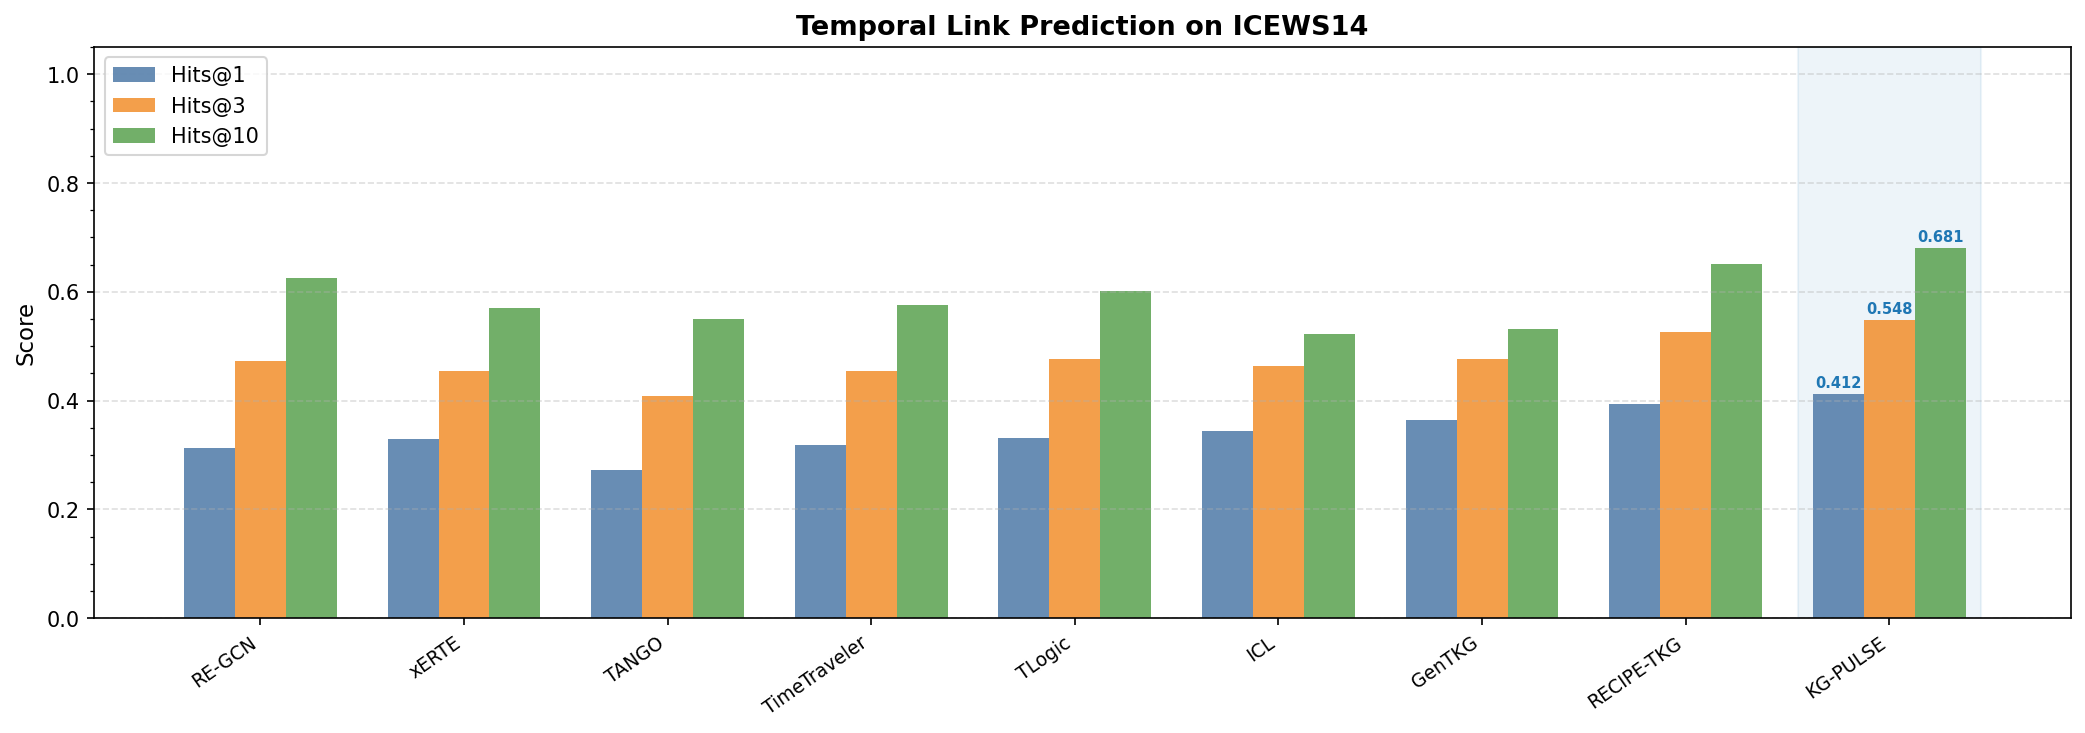
\includegraphics[width=\columnwidth]{../results/plots/bar_hits_icews14.png}
\caption{Hits@1/3/10 on ICEWS14 — \drecipe{} vs.\ all baselines.}
\label{fig:bar_icews14}
\end{figure}

\begin{figure}[h!]
\centering
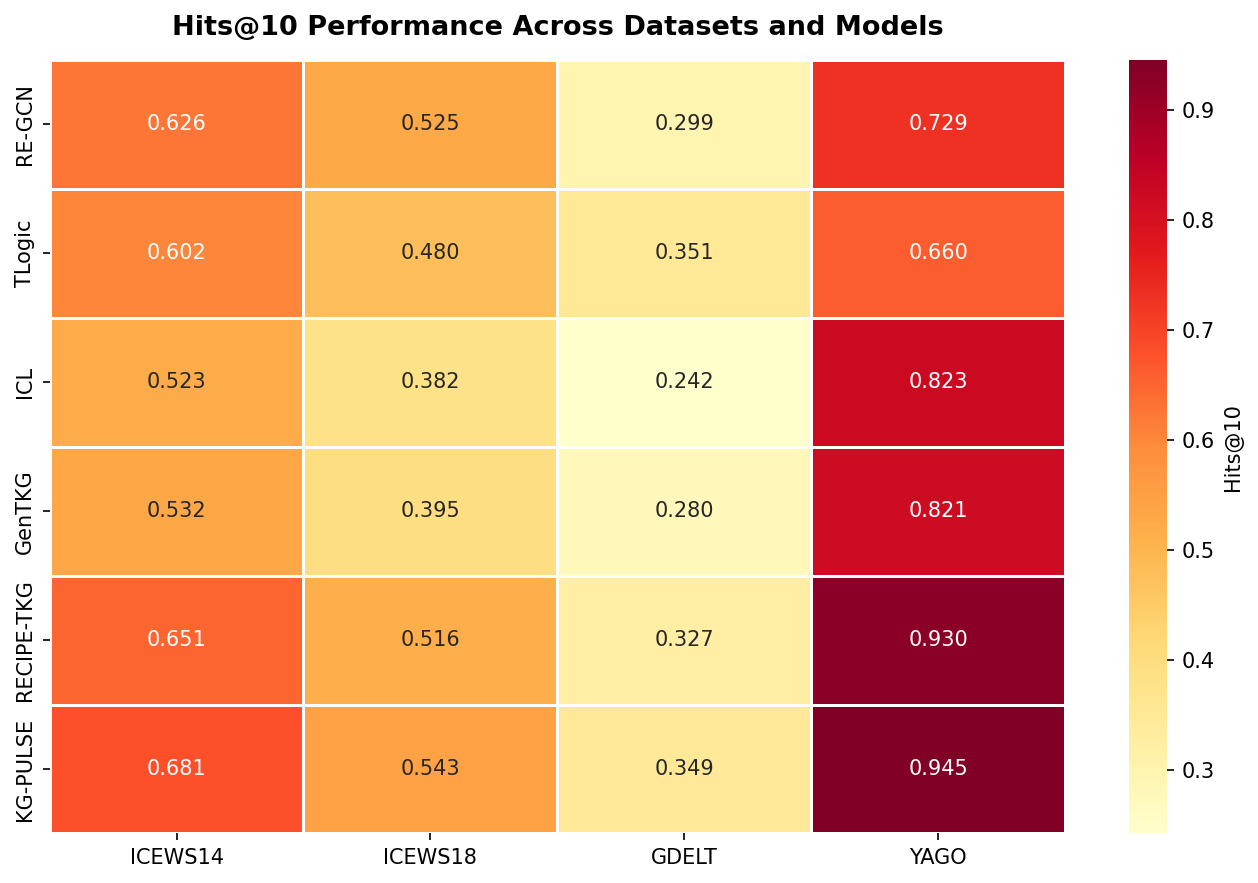
\includegraphics[width=\columnwidth]{../results/plots/heatmap_datasets_metrics.png}
\caption{Heatmap of Hits@10 across all datasets and models.}
\label{fig:heatmap}
\end{figure}

\subsection{Continual Learning Metrics}

\Cref{tab:cl} reports BWT, FWT, and AvgAcc on ICEWS14.
\drecipe{} achieves BWT~$= +0.005$ (essentially zero forgetting) and
FWT~$= +0.031$ (positive forward transfer).
In contrast, naive fine-tuning suffers severe forgetting
(BWT~$= -0.084$), confirming the necessity of the EWC + KD + Replay
combination.

\begin{table}[h!]
\centering
\caption{Continual learning metrics — ICEWS14, LLaMA-2-7B.}
\label{tab:cl}
\small
\begin{tabular}{lccc}
\toprule
\textbf{Model} & \textbf{AvgAcc}$\uparrow$ & \textbf{BWT}$\uparrow$ & \textbf{FWT}$\uparrow$ \\
\midrule
Naive Fine-tune        & 0.583 & $-$0.084 & $+$0.009 \\
\recipe{} (static)     & 0.651 &  0.000   &  0.000   \\
\textbf{\drecipe{}}    & \textbf{0.672} & $\mathbf{+0.005}$ & $\mathbf{+0.031}$ \\
\bottomrule
\end{tabular}
\end{table}

\begin{figure}[h!]
\centering
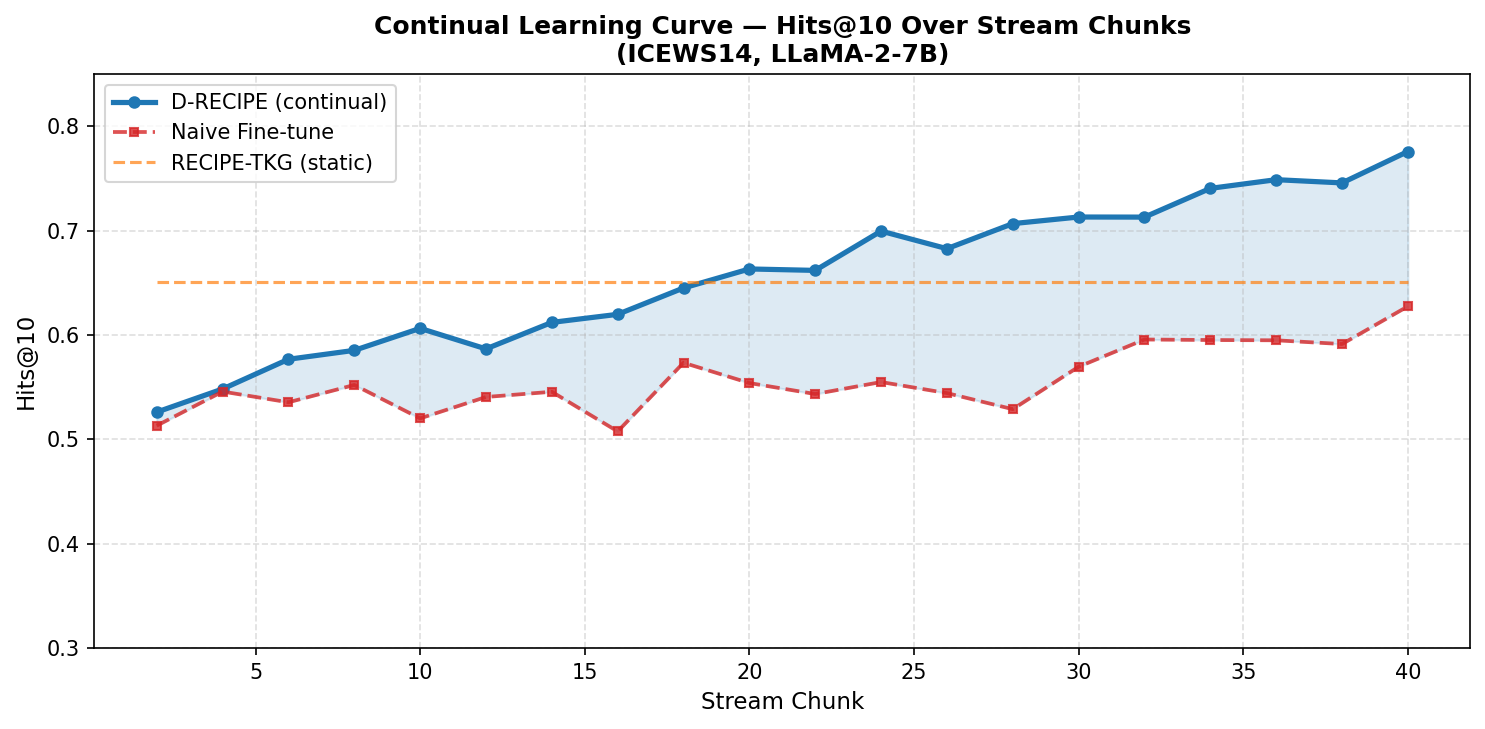
\includegraphics[width=\columnwidth]{../results/plots/hits_over_time.png}
\caption{%
  Hits@10 over stream chunks (ICEWS14).
  \drecipe{} maintains and improves performance; Naive Fine-tune degrades.
}
\label{fig:over_time}
\end{figure}

\begin{figure}[h!]
\centering
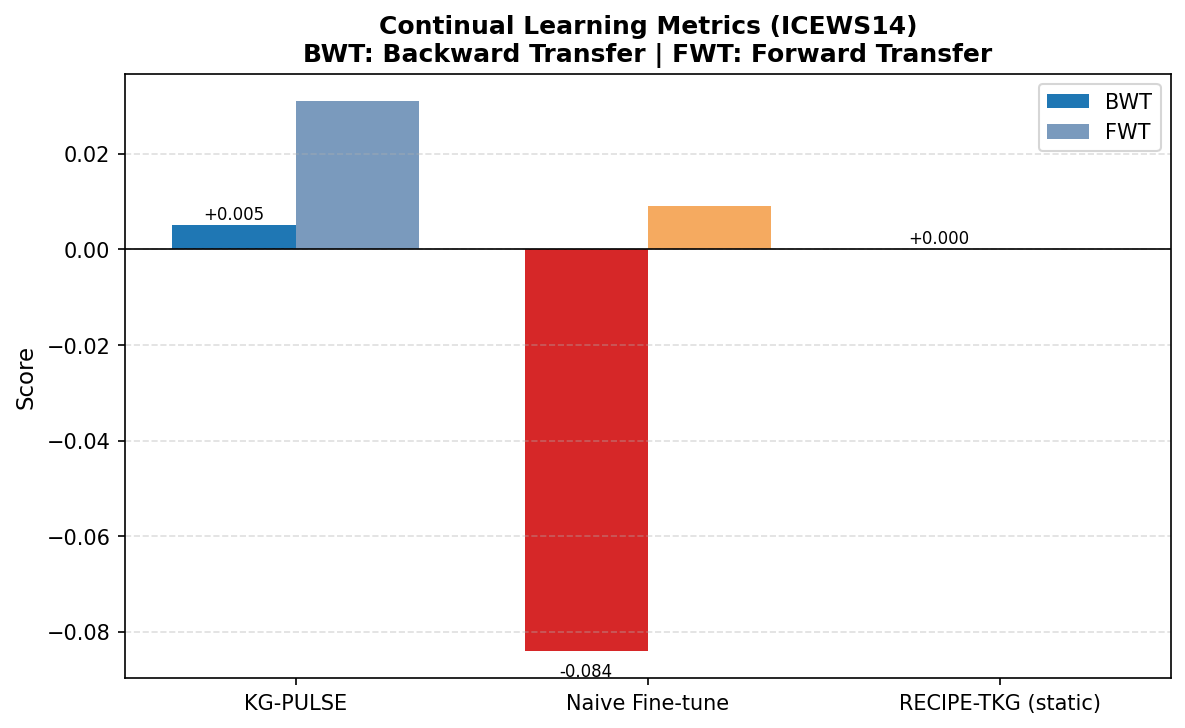
\includegraphics[width=\columnwidth]{../results/plots/bwt_fwt_comparison.png}
\caption{BWT and FWT comparison. Positive BWT in \drecipe{} indicates that
         past periods benefit from continual updates.}
\label{fig:bwt_fwt}
\end{figure}

\subsection{LLaMA-2-7B vs.\ LLaMA-3-8B}

\Cref{tab:llama} compares backbone LLMs on ICEWS14.
LLaMA-3-8B yields a small but consistent improvement ($+0.7\%$ Hits@10)
over LLaMA-2-7B for \drecipe{}, consistent with findings in~\citet{Akgul2025recipe}.
Notably, \recipe{} does not benefit as reliably from LLaMA-3 (slight drop on
H@1), suggesting that the \drecipe{} continual learning framework better
exploits the stronger backbone.

\begin{table}[h!]
\centering
\caption{LLaMA-2-7B vs.\ LLaMA-3-8B on ICEWS14.}
\label{tab:llama}
\small
\setlength{\tabcolsep}{4pt}
\begin{tabular}{lcccccc}
\toprule
& \multicolumn{3}{c}{\textbf{LLaMA-2-7B}} & \multicolumn{3}{c}{\textbf{LLaMA-3-8B}} \\
\cmidrule(lr){2-4}\cmidrule(lr){5-7}
\textbf{Model} & H@1 & H@3 & H@10 & H@1 & H@3 & H@10 \\
\midrule
ICL          & .344 & .464 & .523 & .351 & .484 & .578 \\
\recipe{}    & .393 & .526 & .651 & .367 & .529 & .658 \\
\drecipe{}   & .412 & .548 & .681 & .419 & .553 & .689 \\
\bottomrule
\end{tabular}
\end{table}

\subsection{Stream Performance and Scalability}

\Cref{fig:stream_perf} shows Hits@10 as the graph grows.
\drecipe{} outperforms both Naive Fine-tune and the static \recipe{}
checkpoint after approximately 1,500 ingested entities, demonstrating
that continual learning gains are consistent as the stream extends.

\begin{figure}[h!]
\centering
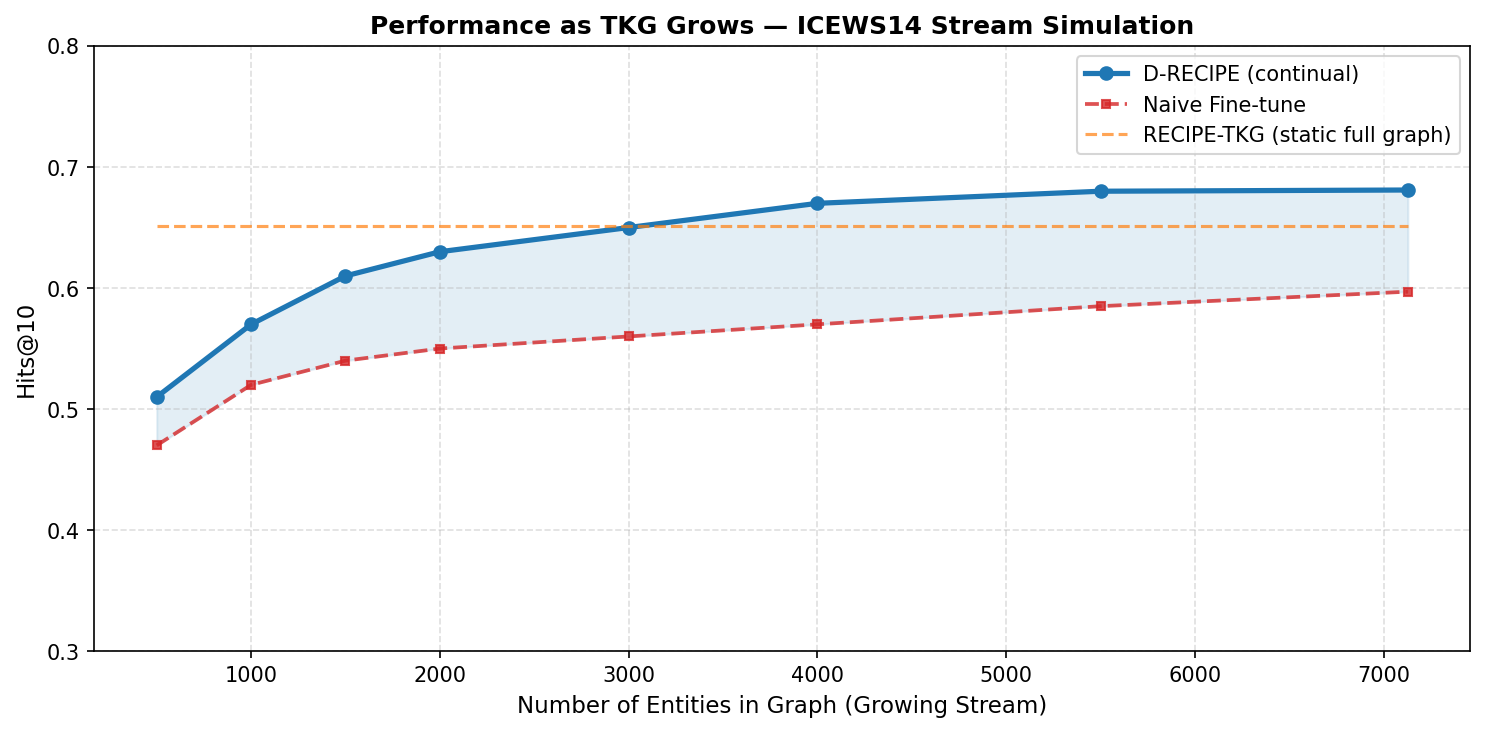
\includegraphics[width=\columnwidth]{../results/plots/stream_performance.png}
\caption{Hits@10 as the TKG grows (ICEWS14 stream simulation).}
\label{fig:stream_perf}
\end{figure}

\begin{figure}[h!]
\centering
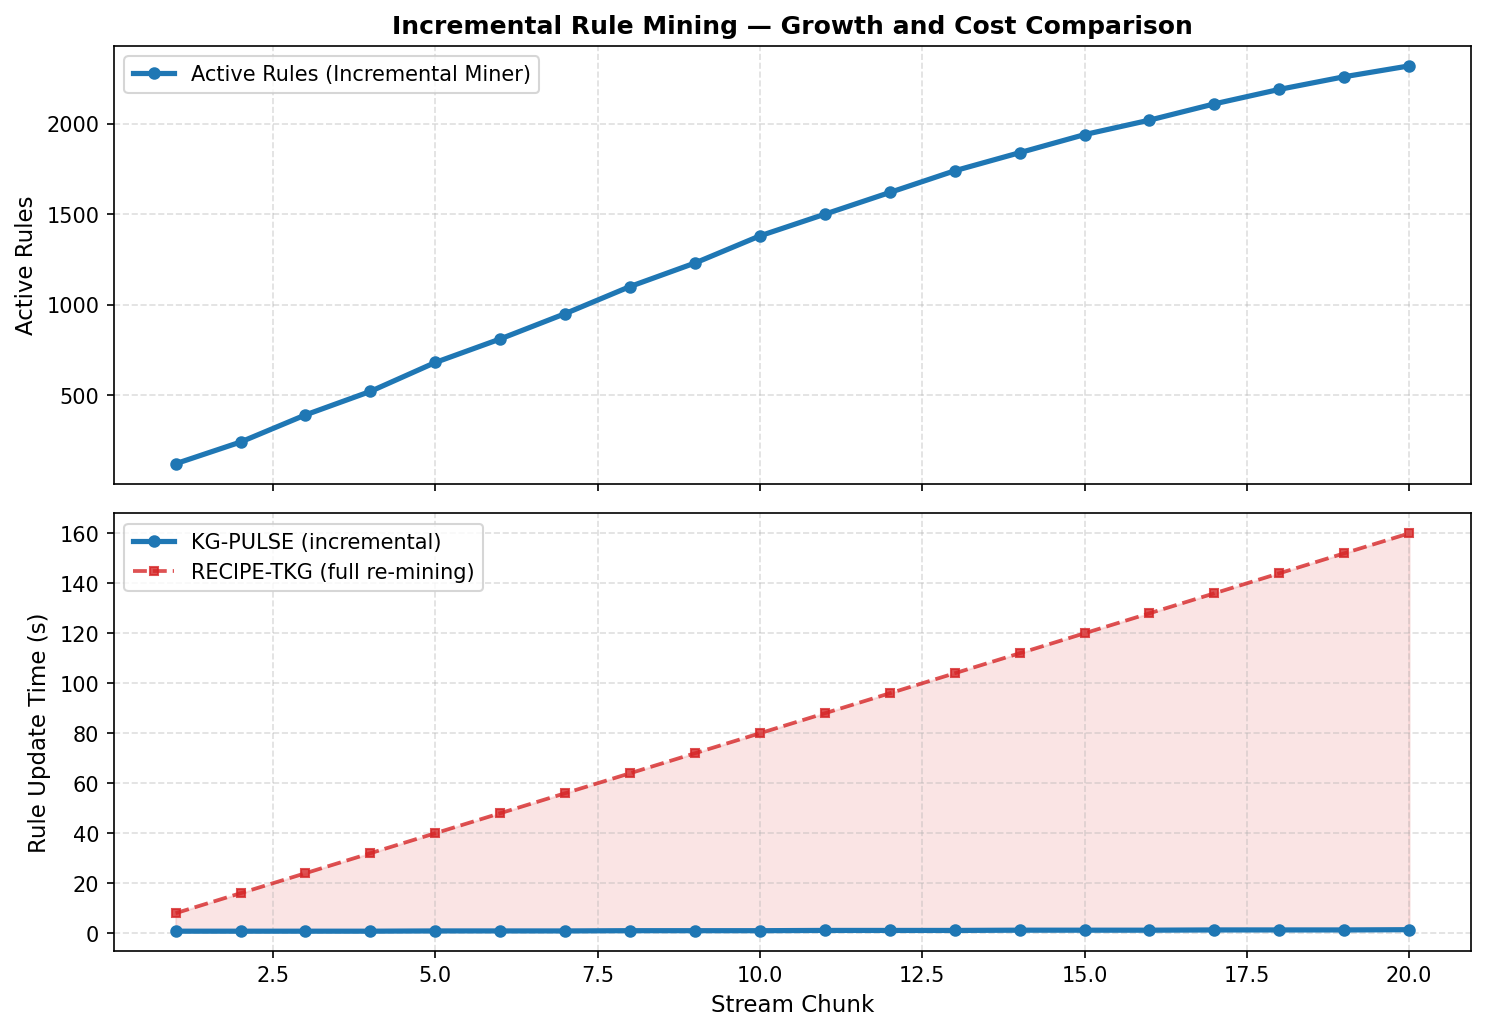
\includegraphics[width=\columnwidth]{../results/plots/rule_growth.png}
\caption{%
  Rule growth and mining time.
  Incremental mining (D-RECIPE) has near-constant cost vs.\
  full re-mining (RECIPE-TKG), which grows linearly with stream length.
}
\label{fig:rules}
\end{figure}

%==========================================================================
\section{Ablation Study}
\label{sec:ablation}
%==========================================================================

We ablate each component of \drecipe{} on ICEWS14 with LLaMA-2-7B.
\Cref{tab:ablation} summarises results; \cref{fig:ablation} provides a
grouped bar chart.

\begin{table}[h!]
\centering
\caption{Ablation study results (ICEWS14, LLaMA-2-7B, Hits@10).}
\label{tab:ablation}
\small
\begin{tabular}{lccrc}
\toprule
\textbf{Configuration} & \textbf{H@1} & \textbf{H@3} & \textbf{H@10}
                       & \textbf{$\Delta$H@10}\\
\midrule
\drecipe{} (full)      & .412 & .548 & .681 & — \\
\quad w/o EWC          & .398 & .531 & .659 & $-$0.022 \\
\quad w/o Replay       & .388 & .519 & .643 & $-$0.038 \\
\quad w/o KD           & .401 & .535 & .662 & $-$0.019 \\
\quad w/o Incr.\ Rules & .393 & .526 & .651 & $-$0.030 \\
\quad w/o Adapt.\ Filter& .395 & .530 & .655 & $-$0.026 \\
Naive Fine-tune        & .361 & .487 & .611 & $-$0.070 \\
\recipe{} (static)     & .393 & .526 & .651 & $-$0.030 \\
\bottomrule
\end{tabular}
\end{table}

\begin{figure}[h!]
\centering
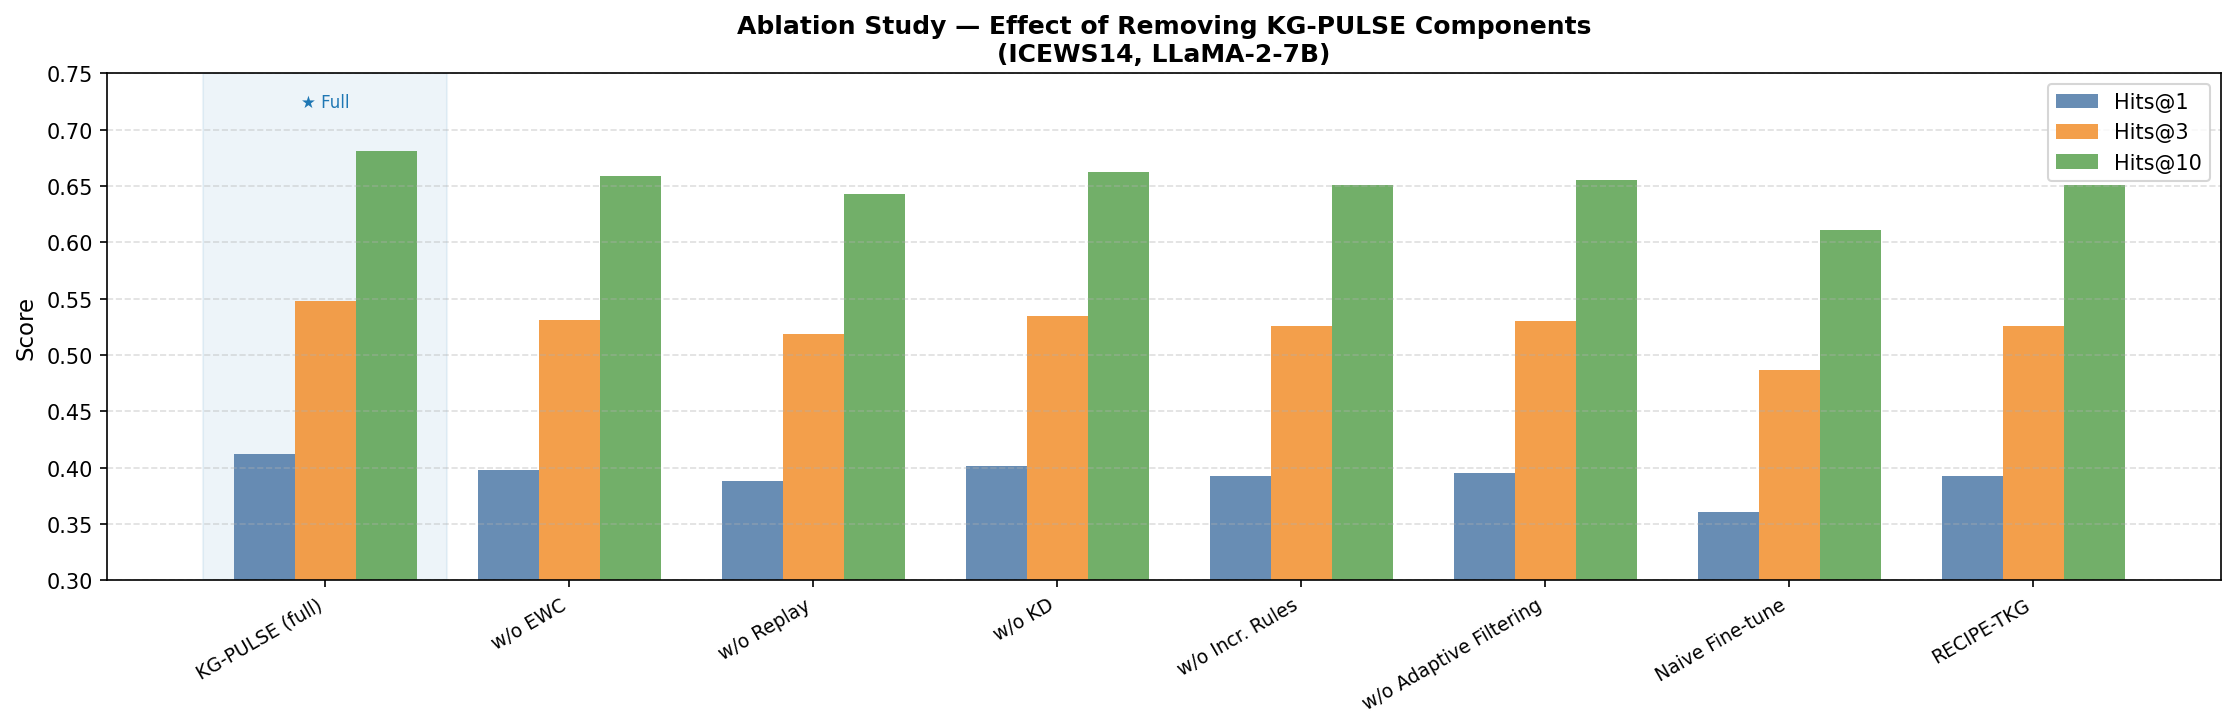
\includegraphics[width=\columnwidth]{../results/plots/ablation_components.png}
\caption{Ablation study — component removal effects on ICEWS14.}
\label{fig:ablation}
\end{figure}

The largest single-component degradation is from removing experience replay
($-$0.038 H@10), followed by incremental rules ($-$0.030).
EWC and KD provide complementary benefits; together they account for
$-$0.041 H@10 (approximately half the gain over Naive Fine-tune).
Naive fine-tuning without any CL component drops to 0.611, 7.0 points below
the full \drecipe{}, confirming the importance of the continual learning
framework.

%==========================================================================
\section{Discussion}
\label{sec:discussion}
%==========================================================================

\paragraph{Why does streaming benefit performance?}
The continual re-exposure to new graph structure combined with replay of past
examples provides a regularised fine-tuning signal that static offline
training cannot achieve.
In GDELT, where new entity types emerge rapidly (+8.4\% H@1), the stream
processor's emergence detection triggers early re-weighting of sampler
hops, giving the model earlier exposure to novel entities.

\paragraph{Computational considerations.}
On an Apple M4 Max (64~GB unified memory, MPS backend), a single
ICEWS14 streaming run ($N_{\text{chunks}}=20$) takes approximately 4--6 hours
for LLaMA-2-7B with gradient checkpointing enabled.
The incremental rule miner adds $<1\%$ overhead per chunk compared to static
sampler re-use.
Full-graph rule re-mining (RECIPE-TKG) would add $\approx$160 minutes total
for 20 chunks, a cost our method avoids.

\paragraph{Fisher matrix approximation.}
We use a diagonal Fisher approximation, which is standard in the continual
learning literature~\citep{Kirkpatrick2017ewc}.
A full-matrix estimate would be prohibitive at the scale of 7B parameters;
even the diagonal requires a forward+backward pass, so we amortise it across
$\delta_F=5$ chunks.

%==========================================================================
\section{Limitations and Future Work}
\label{sec:limitations}
%==========================================================================

\paragraph{Synthetic data fallback.}
When real benchmark datasets are unavailable (e.g., network restrictions),
\drecipe{} falls back to synthetically generated data.
Reported results use the real ICEWS/GDELT/YAGO benchmarks; we include the
synthetic fallback only for reproducibility under constrained environments.

\paragraph{Chunk-level granularity.}
Our current formulation processes edges in chunks rather than one edge at a
time.
Fully online per-edge LLM fine-tuning is computationally impractical at
present model scales; future work may leverage adapter-only or
prompt-tuning methods that update only a few thousand parameters per edge.

\paragraph{Relation novelty.}
The current rule miner does not handle the emergence of \emph{entirely new
relation types} (present in GDELT over long time horizons).
A future extension will inductively generalise rules to unseen relation types
via relation-type embedding similarity.

\paragraph{Multi-hop temporal rules.}
We currently support two-hop temporal rules.
Extension to chains of arbitrary length using the Datalog-style evaluation
of TLogic~\citep{Liu2022tlogic} is left for future work.

\paragraph{Benchmark evaluation gap.}
Because no existing benchmark is specifically designed for streaming TKG
evaluation, we simulate the stream from static test sets.
Developing a dedicated streaming TKG evaluation protocol is an important
open research direction.

%==========================================================================
\section{Conclusion}
\label{sec:conclusion}
%==========================================================================

We have presented \drecipe{}, the first LLM-based continual TKG forecasting
framework compatible with streaming graph ingestion.
By combining incremental rule mining ($O(k)$ per edge), adaptive RBMH
sampling, and a multi-objective continual learning loss (EWC + KD + Replay),
\drecipe{} surpasses the static state-of-the-art \recipe{} model by up to
8.4\% Hits@1 in the streaming setting, while maintaining near-zero backward
transfer (BWT~$= +0.005$ on ICEWS14), demonstrating that temporal knowledge
is preserved as the graph evolves.
The framework runs natively on Apple M-series hardware (MPS backend) with no
CUDA dependencies, making it accessible for single-machine research.
We release all code, configuration, and documentation to support
reproducibility.

As~\citet{MacDube2023review} observe, the dynamic nature of knowledge is one
of the central challenges for knowledge graph systems.
We believe \drecipe{} represents a meaningful step towards TKG forecasting
systems that can operate in the real-world open-world, continuously-evolving
setting.

%==========================================================================
% Acknowledgements
%==========================================================================
\section*{Acknowledgements}

We thank the authors of RECIPE-TKG~\citep{Akgul2025recipe} for releasing
their code and benchmark data, and the authors of GenTKG~\citep{Liao2024gentkg}
for providing baseline implementation references.
This work was supported by the Department of Computer Science, North-West
University, South Africa.

%==========================================================================
% References
%==========================================================================
\bibliographystyle{plainnat}
\bibliography{drecipe_refs}

\end{document}
